\chapter{Design: How David and I applied these tools to make the REIXS spectrometer optical design}
\section{Application to spectrometer design}
Up to this point, we have covered the theoretical foundation of grating efficiency, introduced new software tools for performing efficiency calculations, and used these tools to understand how various parameters and conditions affect a grating's performance.  We have also validated the calculation results by comparing against efficiency measurements on a set of  real-world gratings.

In this chapter, we describe how we applied these results to the design of the soft x-ray emission spectrometer for the REIXS beamline at the Canadian Light Source.

\subsection{Design goals}
The REIXS beamline at the CLS is intended to facilitate a high-throughput user science program in the field of material science.  Academic users apply for beamtime through a peer-reviewed proposal process, and are awarded shifts on the beamline based on the comparative scientific merit of their proposal.  These shifts typically range from as short as eight hours, to as long as a week.  (A fraction of the total beamtime is set aside for industrial clients, who purchase beamtime or analytical services from the facility.)

For the endstation designers, the challenge of supporting a general user program led to some high-level goals.  We wanted to ensure that the spectrometer would be an adaptable ``work horse'', applicable to a wide variety of emission experiments.  High efficiency was important to minimize the time required for individual scans, maximize the total user throughput of the beamline, and make the spectrometer useful for dilute samples.  At the same time, we wanted to push the resolving power of the machine to be competitive with the highest-resolution spectrometers currently in existence.  (If we could somehow exceed world-record resolution without sacrificing these other goals, there could even be a possibility of making new discoveries that would be invisible on existing beamlines.)

The design goals were also influenced by the current focus of the material science research group in the Physics Department at the University of Saskatchewan, with interests in organic biomaterials (DNA and peptides), organic semiconductor and photonic materials, and transition metal oxides.

The performance of the spectrometer was to be derived from the following key strengths: \cite{Mui06}
\begin{enumerate}
\item Superior optimization of the design to specific spectral windows of interest, for   analysis of materials containing
\begin{itemize}
\item silicon (Si L $\beta$ emission edge, 92 eV), 
\item carbon (C K $\alpha_1$ emission edge, 277 eV), 
\item nitrogen (N K $\alpha_1$ emission edge, 392 eV) and 
\item oxygen (O K $\alpha_1$ emission edge, 525 eV), 
\end{itemize}
while maintaining acceptable performance for 
\begin{itemize}
\item soft x-ray transitions in transition metals (L $\alpha,\beta$ and M $\alpha,\beta$ edges, 600 eV - 1100 eV).
\end{itemize}
\item A focus on best achievable performance, instead of a compact, mechanically simple or low-budget design.
\item A mechanical design allowing for superior alignment and calibration.
\item An optical design based on careful, knowledgeable balancing of the tension between efficiency and resolution.
\end{enumerate}
The final key strength was achieved through close teamwork with David Muir, who used ray tracing techniques to quantify and optimize the resolution of our design.  His full analysis of spectrometer focussing and resolving power is published in his M.Sc. thesis; some relevant areas of overlap are summarized briefly in this chapter, but for full details we would refer interested readers to Reference \cite{Mui06}.

Together, we set a quantitative goal for both efficiency and resolution: 10\% efficiency and a resolving power of 2000 at all the emission lines of interest.  The design constraints were set by the maximum mechanical length of the spectrometer (the physical space available on the beamline floor was limited to 3m at the time) and the endstation budget of approximately \$1 million.
\subsection{Comparative examples}
Before starting work on the REIXS spectrometer, we examined the designs of existing spectrometers at facilities around the world.  (Given that we had never designed a soft x-ray spectrometer before, this was a natural starting point, and one that would ensure that -- for lack of original ideas -- we would design a machine at least as good as any other in existence.)

We analyzed a variety of machines covering a range of design goals, from mechanical compactness and simplicity of grating/detector motion, to maximum resolution.  It turned out to be difficult to accurately compare the stated resolution of the different machines, due to differences in the resolving power criterion and variability in the spatial resolution of their detectors.  David resolved this by modelling the optical layout and conducting ray-trace simulations for each one.  To decouple the detector performance -- which affects the final resolution but is not related to the optical design -- from the pure optical performance, we simulated them using a standardized detector with a hypothetical spatial resolution of 20 um.  

Figure \ref{4a} shows this normalized comparison of spectrometer resolution.  For machines offering a choice of gratings, the plot shows the performance attainable by each grating.  Among these machines are the SXF spectrometer from Beamline 8.0.1 at the Advanced Light Source \cite{Jia95} (Figure \ref{1d}); another Rowland circle spectrometer, the commercially-available Gammadata XES350 \cite{xes350}; and several recent variable line spacing (VLS) designs.  Unfortunately, we were not able to compare the efficiency for these designs, because the exact grating groove parameters are rarely known or published.
          
\begin{figure}[htbp] %  figure placement: here, top, bottom, or page
   \centering
   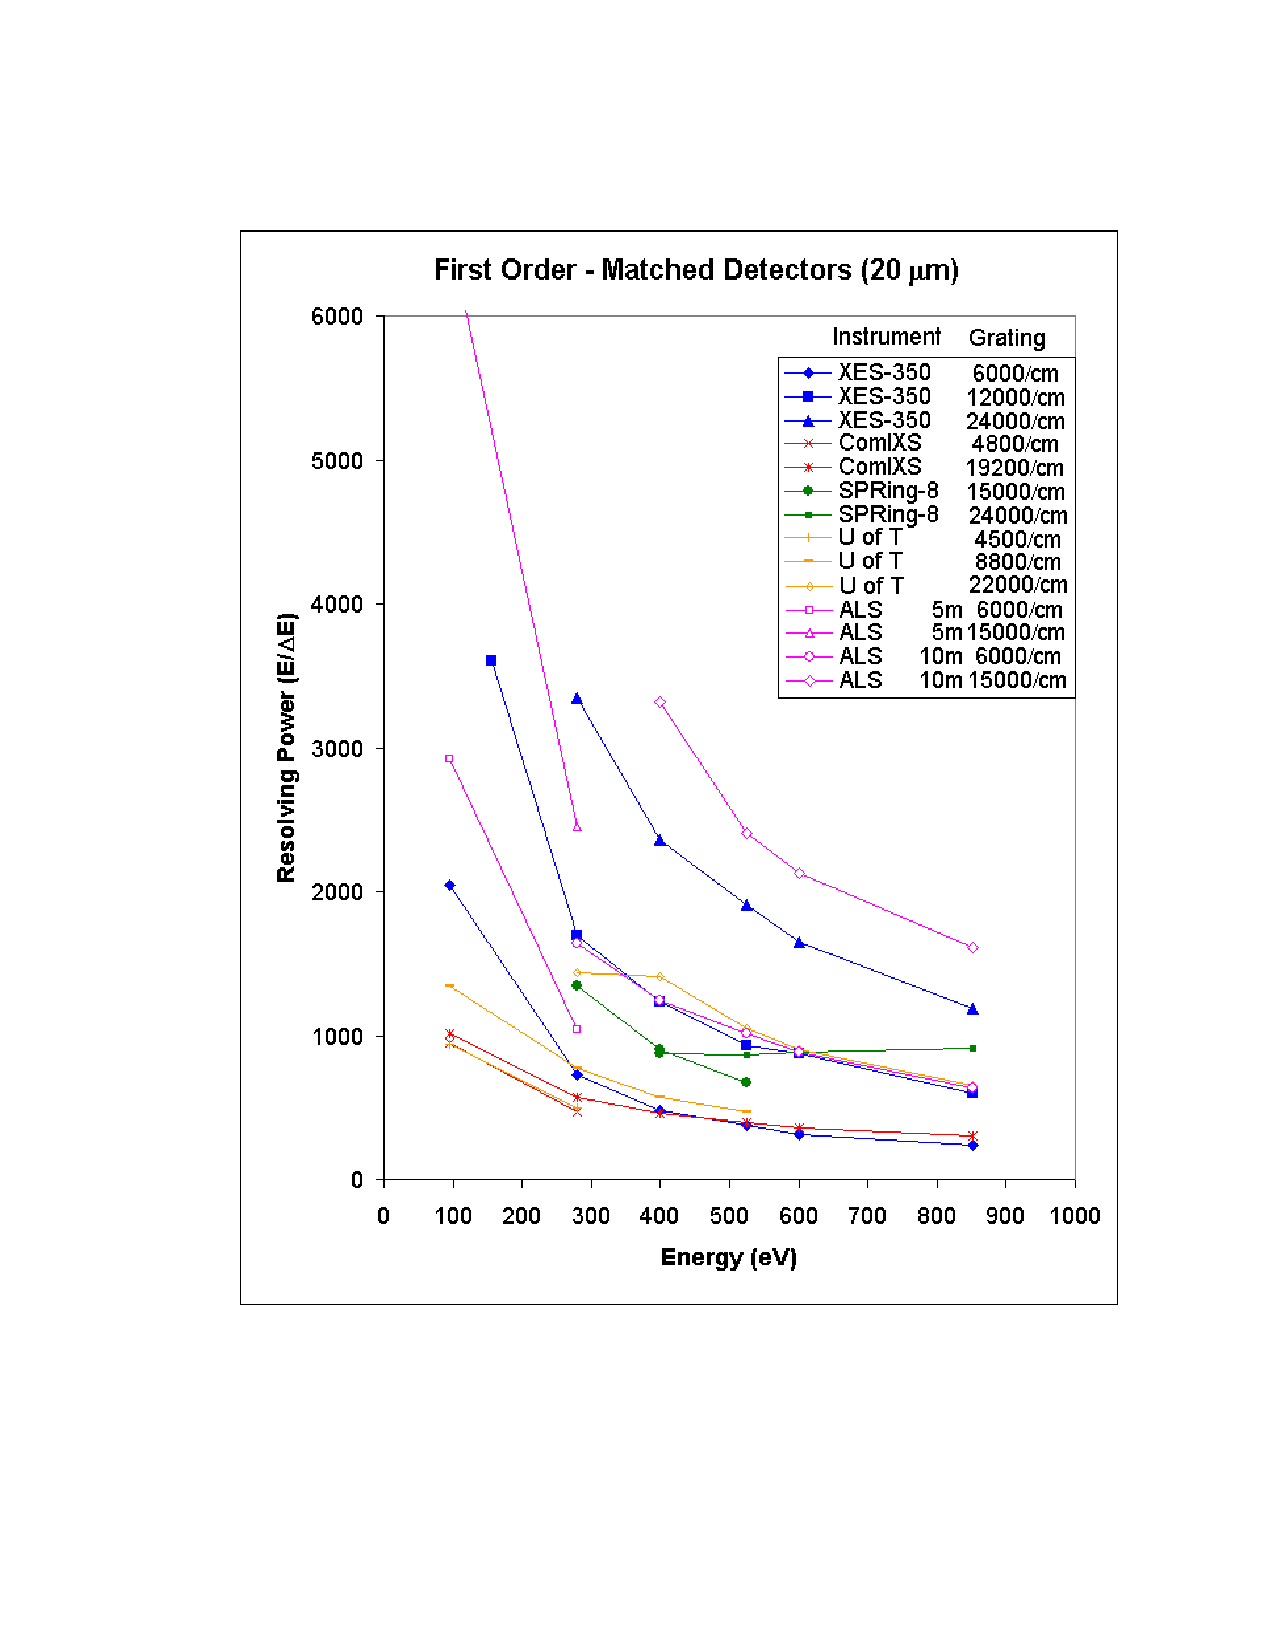
\includegraphics[width=4in]{Chapter4/4a_resolution/4a.pdf} 
   \caption[Resolving power performance comparison of existing spectrometer designs, calculated with all detectors having a 20 um pixel size.]{Resolving power performance comparison of existing spectrometer designs, calculated with all detectors having a 20 um pixel size. The legend specifies the spectrometer and grating choice (size and/or line density).  Reprinted from Reference \cite[Figure 3.2]{Mui06}}
   \label{4a}
\end{figure}

\section{Design Process}
The first step in the design process was to choose the focussing configuration of the spectrometer.  Based on our comparison of existing designs, we selected the Rowland circle configuration for the reasons in Section \ref{rowlandVsVLS}.

To determine the number of grating choices to offer, we started by assuming one grating optimized for each emission line of interest: Si (92 eV), C (277 eV), N (392 eV), O (525 eV), and the transition metal range (600 - 1100 eV) optimized for Fe (725 eV).  Eventually, after completing the subsequent steps in the design process, we found that we could merge the medium energy gratings (277, 392 eV) and high energy gratings (525, 725 eV), since there was considerable overlap in their performance.  This allowed us to add a fourth grating, intended to cover a large energy range with extremely high efficiency, for studying dilute samples; we called this one the ``impurity'' (IMP) grating.  Later, we added two more gratings, intended to offer impressively high resolution, in the medium energy (HRMEG) and high energy (HRHEG) range; these 3rd order gratings are described in Section \ref{3rdOrderDesign}.

\renewcommand{\arraystretch}{1.3}
\begin{table}[h]
   \centering
   \topcaption{Gratings chosen for the REIXS spectrometer, with their target energies used for optimization, the energy ranges they will be able to cover, and the final optimized grating parameters}
   {\footnotesize
 \begin{tabular}{@{} llccccc@{}} % Column formatting, @{} suppresses leading/trailing space
\toprule
        Grating    & Optimization& Energy& Groove Density & Incidence & Coating & Blaze\\
        & Energy (eV) & Range (eV) & (lines/mm) & Angle ($\deg$) & &Angle ($\deg$)\\
\toprule
      &&$1^\textrm{st}$ order&&&&\\
\midrule
Low Energy (LEG) & 92 eV (Si) & 30 - 300&600&86&Au&1.85\\
Impurity (IMP) & \emph{400 eV (N)} & 75 - 750&900&87&Ni&1.11\\
Medium Energy (MEG) & 400 eV (N) & 250+&1200&88&Ni&1.48\\
High Energy (HEG) & 725 eV (Fe) & 400+&2000&88&Pt&1.52\\
&&&&&&\\
\toprule
 & &$3^\textrm{rd}$ order&&&&\\
\midrule
High Res Medium Energy (HRMEG) & 280 eV (C) & 280+&1800&88&Ni&4.85\\
High Res High Energy (HRHEG) & 725 eV (Fe) & 525+&2600&88.25&Pt&4.05\\
\bottomrule
   \end{tabular}
   }
   \label{gratings-table}
\end{table}
\renewcommand{\arraystretch}{1.2}

The next step was to determine the grating parameters (line density, profile) and the optical geometry (incidence angle, distances, grating radii, etc.), subject to the focussing constraints, to reach our target resolution and efficiency.
% TODO TODO Table \ref{4b} TODO describes all of the overlapping parameters in a Rowland circle spectrometer that affect resolution, geometric efficiency, and/or grating efficiency; almost universally, increases in one goal result in decreases in the others.

Because of the inherent tension between resolution and efficiency, attempts to establish the grating parameters prompted a carefully-choreographed, swashbuckling duel between the Forces For Efficiency (FFE) and the United Resolutionary Front (URF).  This battle became an iterative process, involving a degree of trial-and-error and continuous refinement.  In retrospect, the design process we would recommend for future designs is summarized in Figure \ref{4c}.  The final grating parameters that affect the efficiency are shown in Table \ref{gratings-table}.

\begin{figure}[htbp] %  figure placement: here, top, bottom, or page
   \centering
   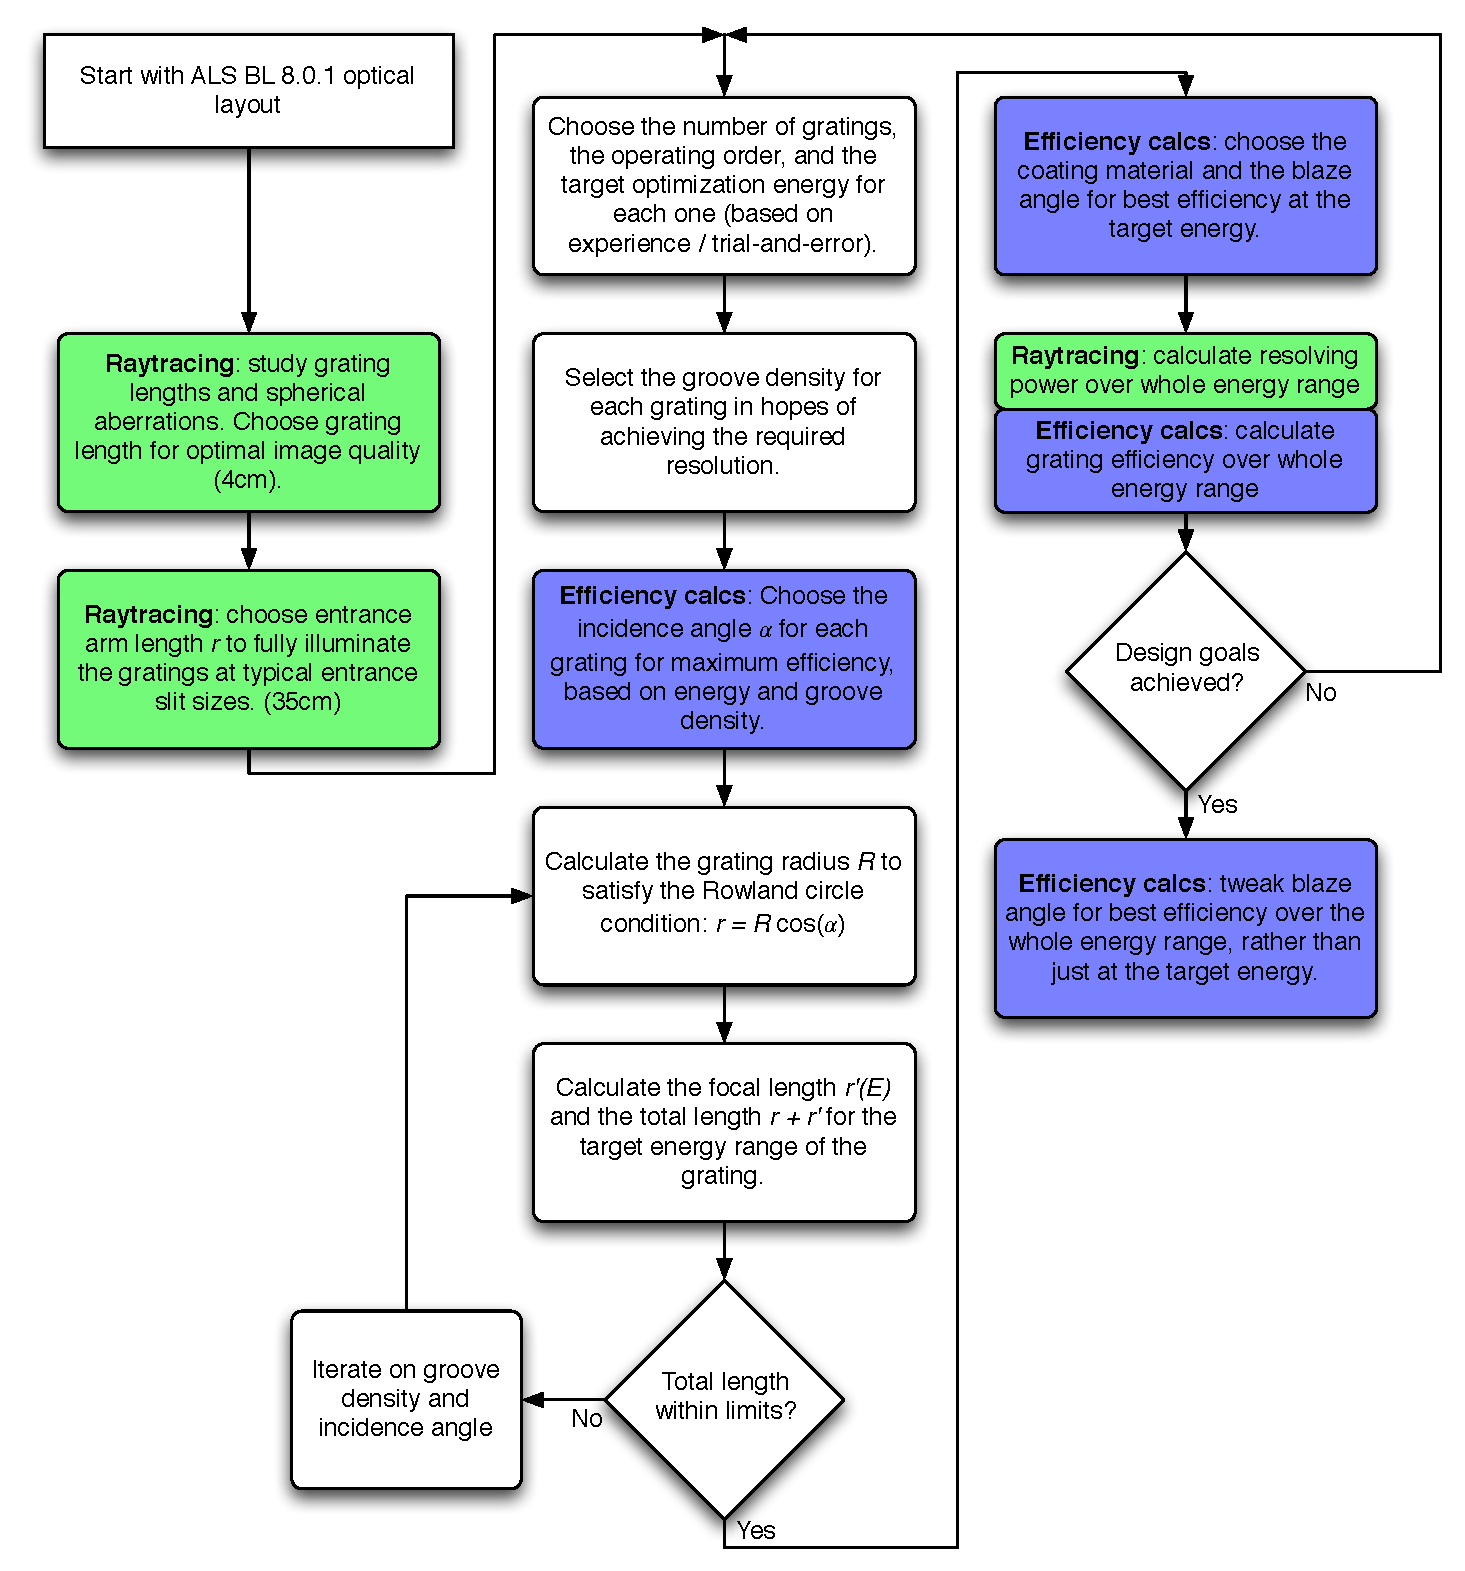
\includegraphics[scale=0.6]{Chapter4/4c_process/4c_mine.pdf} 
   \caption{Approximation of the process used to design the optics of the REIXS spectrometer.}
   \label{4c}
\end{figure}

\subsection{Justification of design choices}
\subsubsection{Rowland circle vs. VLS design} 
\label{rowlandVsVLS}
We mentioned in Chapter 2 that spectrometer optics must focus as well as disperse light.  Some of the designs we surveyed achieved this using VLS gratings, while others employed spherical gratings in the ``Rowland circle'' configuration.  Fortunately, this provided us with a good basis for comparison.

According to Reference \cite{Mui06}, the main advantage of VLS gratings is to control the shape of the focal curve -- the path in space that the detector must travel along to keep the spectrometer focussed as a function of energy.  A flat focal curve simplifies the mechanical design, since the detector then only needs to move along one axis.  As Figure \ref{vlsCurves} shows, the VLS correction also shortens the focal curve, so that to handle the same energy range, a spectrometer can be made more compact.  Unfortunately, a compact focal curve places the detector closer to the grating and inherently reduces the resolution -- as a result, all of the VLS designs we surveyed required very high spatial resolution detectors to maintain just average resolution \cite[Table 3.3]{Mui06}.
% TODO review current leading spectrometers at ESRF, SLS... VLS with very long arms.

The VLS technique can also be used to minimize aberrations (astigmatism, coma, etc.), but these can only be fully corrected at a single energy; for a general-purpose spectrometer, this is not helpful.\footnote{After completing our Rowland circle design, an external consultant attempted to optimize it by adding VLS terms to correct aberrations.  While this worked well at the optimization point of 200 eV, the detector image became heavily defocussed just 50 eV away \cite[Figure 5.1]{Mui06}.} Using VLS corrections also removes the flexibility to operate the spectrometer in higher orders: since the formulas for the correction terms depend on the diffraction order, VLS spectrometers behave erratically outside of their design order.

Figure \ref{vlsImage} compares the detector image of three adjacent energy lines, for a comparable VLS and Rowland circle spectrometer.  While requiring a longer focal curve and more complicated detector motion, the Rowland design offers far higher resolution for the same nominal groove density; it would take a large increase in efficiency-robbing line density for the VLS design to keep up with it.  Therefore, since we were not constrained by physical size\footnote{At least, we were not constrained beyond the 3 meter limit of the beamline space}, we selected a Rowland circle optical layout -- similar to the ALS Beamline 8.0.1 SXF spectrometer, as the basis for our design.

\begin{figure}[p] %  figure placement: here, top, bottom, or page
   \centering
   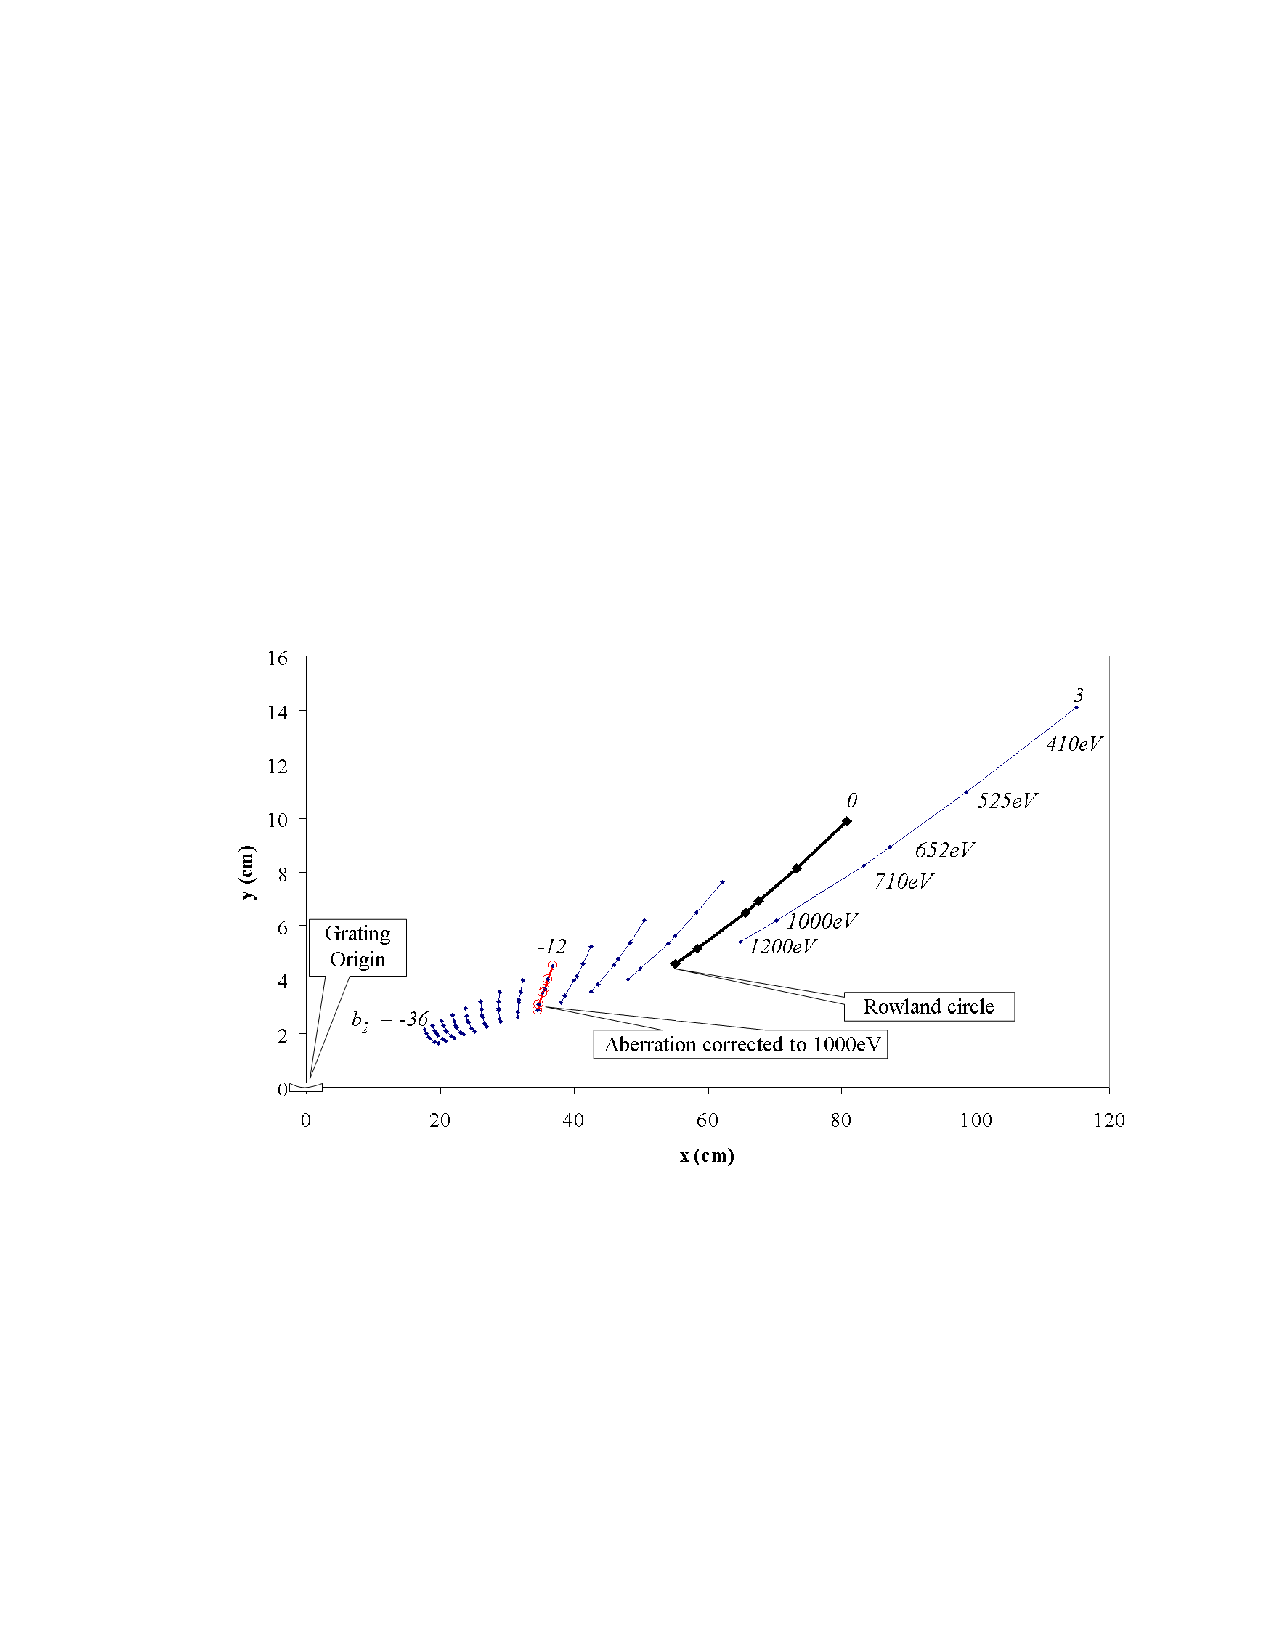
\includegraphics[scale=1.0]{Chapter4/4z_vls/focalCurves_David2_17.pdf} 
   \caption[The focal curve is the path in space the detector needs to move along to maintain focussing as a function of energy.  This plot shows the effect of the $b_2$ VLS correction term.]{The focal curve is the path in space the detector needs to move along to maintain focussing as a function of energy.  This plot shows the effect of the $b_2$ VLS correction term: with a $b_2$ of 0, the focal curve is the same as the Rowland circle focal curve.  A specific $b_2$ value of -12 (highlighted in red) straightens the focal curve, which could simplify the detector mechanics, but also shortens the focal distance and reduces the resolution at the detector.  Reprinted from Reference \cite[Figure 2.17]{Mui06}.}
   \label{vlsCurves}
\end{figure}

\begin{figure}[p] %  figure placement: here, top, bottom, or page
   \centering
   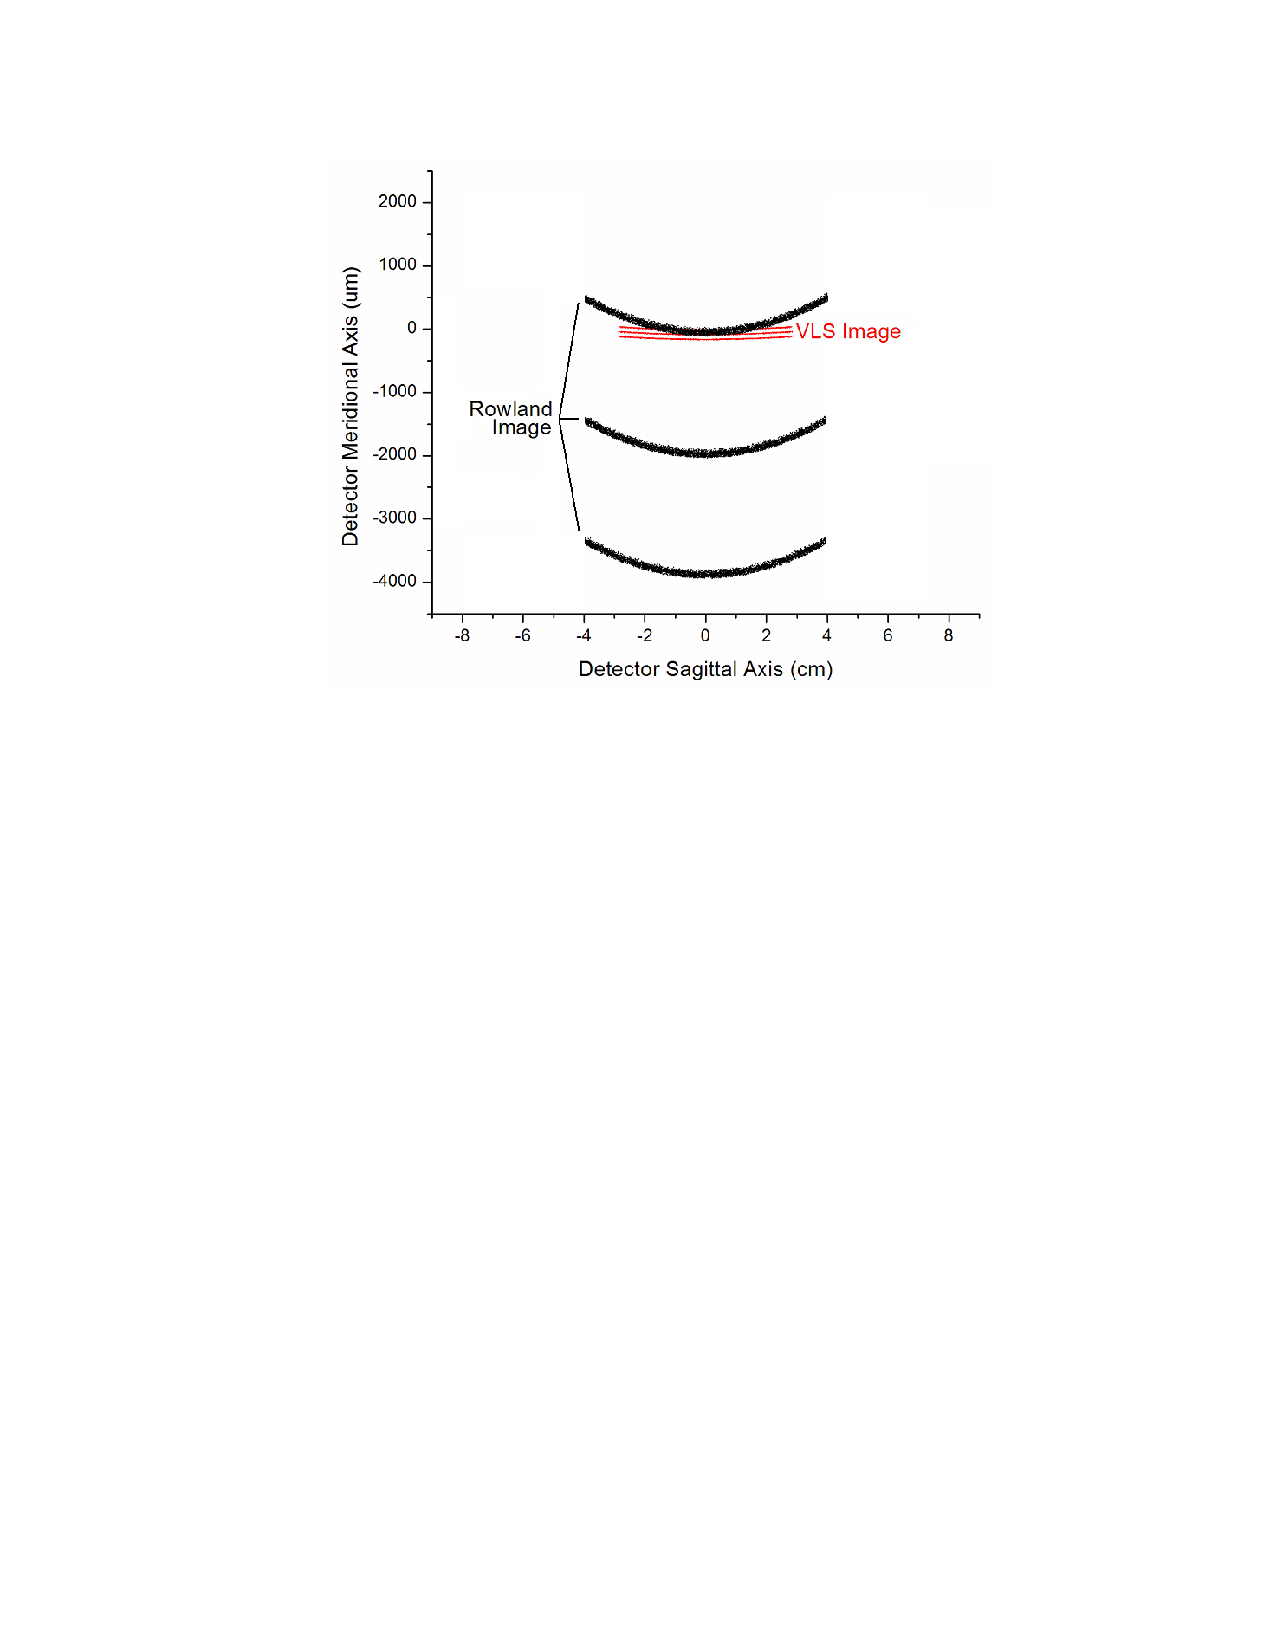
\includegraphics[scale=1.0]{Chapter4/4z_vls/detectorImage_David2_18.pdf} 
   \caption[Variable line space (VLS) corrections reduce aberrations that cause curvature, as seen in these ray-traced detector images of three adjacent emission lines.  However, the increase in resolution due to better focussing is not able to make up for reduced dispersion across the surface of the detector.]{Variable line space (VLS) corrections reduce aberrations that cause curvature, as seen in these ray-traced detector images of three adjacent emission lines.  However, the increase in resolution due to better focussing is not able to make up for reduced dispersion across the surface of the detector, as compared to the Rowland circle alternative. Reprinted from Reference \cite[Figure 2.18]{Mui06}.}
   \label{vlsImage}
\end{figure}

\subsubsection{Choice of profile: blazed vs. rectangular / sinusoidal}
Back in Chapter 4, we saw that optimally blazed gratings have almost double the efficiency of sinusoidal gratings, and even more than that of rectangular gratings (Figure \ref{3c-plot}).  Since the ideal blaze angle is energy-dependent, we saw that this optimization comes at the cost of having an efficiency peak centred on the target energy, and comparably lower efficiency outside the peak.  However, for high groove densities and high optimization energies, the peaks are wide enough to span the entire soft x-ray range.  For low groove densities and low optimization energies -- as would be the situation for the LEG -- the peak bandwidth is smaller, but still easily covers the design energy range of this grating.

For each grating, we selected blaze angles corresponding to the target energies in Table \ref{gratings-table}, according to Equation \eq{blazeAngleEqn}.  We then used the efficiency software to optimize the blaze angle at this energy, using the analytical $\theta_b$ as a starting point.  We then calculated the efficiency curves for these profiles, as well as for optimized sinusoidal and rectangular alternatives, and confirmed that the blazed profile was indeed the clear winner for all the gratings.  (For some of the gratings, we tweaked the blaze angle at the end of the design process, since we were willing to accept a small reduction in efficiency at the target energy in exchange for higher overall efficiency integrated across the whole energy range.)
        
\subsubsection{Ruled versus holographic gratings}
Section \ref{gratingManufacturing} gave an overview of mechanical ruling and holographic grating manufacturing techniques.  To make a pragmatic decision between these two options, we needed to consider the impacts of real-world manufacturing issues.  Common errors which happen during ruling and holographic manufacturing are shown in Figure \ref{4d}.

\begin{figure}[htbp] %  figure placement: here, top, bottom, or page
   \centering
   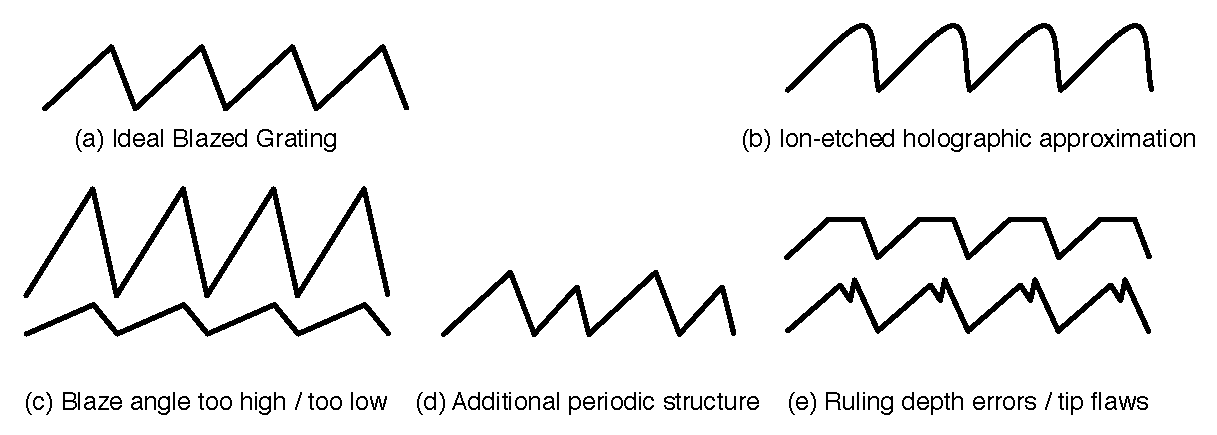
\includegraphics[scale=0.8]{Chapter4/4d_rulingFlaws/4d.pdf} 
   \caption[Common errors in the manufacture of ruled and holographic gratings.]{Common errors in the manufacture of ruled and holographic gratings.  Holographic exposure creates a sinusoidal profile; subsequent ion-etching (b) can only approximate a triangular profile.  Ruled gratings can suffer from blaze angle errors (c), or errors due to the shape and/or depth of the diamond tip (e).  If the ruling engine introduces periodic errors in the groove position, this additional structure (d) superimposes additional diffraction patterns (ghosts).}
   \label{4d}
\end{figure}

Mechanical ruling engines are designed to be precision machines, but they must be carefully set up and operated to avoid errors.  Achieving the specified blaze angle -- critical to efficiency -- must be accomplished during setup by aligning the diamond tip, ruling a test section of the grating, analyzing the resultant blaze angle with a microscope, adjusting the tip, and tediously repeating this process.  Without sufficient quality control, the blaze angle can end up high or low by a few tenths of a degree, which could completely eliminate the blazing advantage.

Another concern is whether the grooves end up uniform, and the groove geometry is maintained, across the entire grating.  This is essential to both the efficiency and the resolution.  If the ruling process creates errors that vary periodically over a series of grooves, this will insert additional periodic structure into the grating and create ``ghosts'' in the final spectrum: an additional diffraction pattern superimposed over the desired one, with intensity peaks again given by the grating equation, but at a different period.  Errors with a period on the same order as the groove spacing create ``Lyman ghosts'', which end up far from the spectral lines.  Errors with periodicities on the order of millimetres create ``Rowland ghosts'', which appear close to and symmetric around the desired spectral lines.

One additional flaw that can occur with ruled gratings happens when the diamond tip fails to penetrate far enough into the metal surface to create the desired profile, resulting in something that looks like Figure \ref{4d} (e).  The profile can also be corrupted by irregularities in the diamond tip, or by bits that break off or are picked up during the ruling process.  (One common manufacturing error is for the tip to pick up a shard of metal, and carry it with it for several thousand trips across the grating; this creates an inefficient stripe across an otherwise acceptable grating.)  Finally, for maximum efficiency, the anti-blaze angle should be as close to 90$\deg$ as possible, but in most cases the shape of the ruling tip forces it to be below 30$\deg$.  (The blazed grating in Figure \ref{3j-1} had an anti-blaze angle of $12.8\deg$.)  According to the theoretical calculations in Figure \ref{3k}, the anti-blaze angle does not start to seriously affect the efficiency until it goes below $\sim$4 times the blaze angle, ie: 5$\deg$ for a blaze angle of 1.5$\deg$.

Holographic gratings overcome many of these disadvantages.  They are not susceptible to ghosting, since their grooves are all formed simultaneously, with a period as regular as the wavelengths of an electromagnetic wave.\footnote{However, modern interferometrically-controlled ruling engines can inscribe grooves with such precision that they have also virtually eliminated ghosting.}  They can also be ruled faster and at lower cost -- mechanical ruling can take weeks for one grating -- so that flaws can be corrected by trial-and-error.  Despite these advantages, holographic gratings  have their own manufacturing challenges.  In some cases, variation in the sinusoidal groove depth happens because the intensity of the interference pattern changes across the width of the grating.  Traditionally, holographic techniques also have not been able to produce groove densities as high as mechanical ruling engines.  The most significant drawback to holographic gratings, however, is their inability to create a true blazed profile, even when using ion etching or the Sheridon method (Figure \ref{4d} (b) ).  For this reason alone, we chose mechanical ruling for all six of the spectrometer gratings.

In future work, it would be helpful to characterize the typical groove shape of real-world ion-etched holographic gratings, and update the grating efficiency software to support this additional profile; this could allow for more informed decision-making on whether to use or reject holographic ruling.

\section{High resolution (3rd order) design}
\label{3rdOrderDesign}
\subsection{Options for reaching extreme resolution}
We mentioned in Section \ref{resolutionGoals} that the two general ways to increase the resolution of a spectrometer design (besides choosing a better detector) are to move the detector further away from the grating, or to increase the angular dispersion of the grating.  Increasing the detector distance requires adjustments to the focussing scheme, and severely reduces geometric efficiency.\footnote{In a Rowland circle design, ray trace testing \cite{Mui06} showed us that the geometric efficiency is proportional to the inverse cube of the detector distance. The reduction in saggital angle captured by the detector causes the first reduction. The grating radius $R$ needs to be increased to maintain focussing,  and with spherical gratings, this further increases the saggital dispersion.  The entrance distance $r$ also needs to be increased, causing a reduction in the solid angle captured by the grating. This could be compensated by increasing the grating size, but the total grating size is constrained by limits on spherical aberration.}  This option also is not an option when the constraints on the machine size have been reached.  The other method -- increasing the angular dispersion -- can either be achieved using the groove density, or the diffraction order.  As we saw in Figure \ref{3e-2}, higher groove densities reduce the grating efficiency, and are also constrained by manufacturing limits.\footnote{While some ruling engines can now reach extremely high groove densities approaching 10~000 lines/mm, the groove quality and accuracy suffers.  For soft x-ray gratings, 3~000 lines/mm seems to be a current effective limit for both mechanical and holographic ruling.}

So this leaves three related questions for a designer trying to achieve extreme resolution: what do you when you have hit the machine size limit \emph{and} the groove density manufacturing limit? Does taking these parameters all the way to their limits actually the optimal solution for maintaining efficiency at high resolution?  What are the consequences of designing intentionally for a higher diffraction order?

All existing soft x-ray spectrometers seem to be designed for 1st order operation, based on the assumption that diffraction efficiencies in higher orders are too low to be useful.  (We have seen users force some Rowland circle designs into 2nd order, when trying to tease out higher resolution.)  Although it had never been done before, our survey of efficiency trends hinted that it might actually be more efficient to use gratings in 3rd order, than to triple their groove density or extend the machine size.  Based on these results, we attempted to add ultra-high-resolution capabilities to the REIXS spectrometer, by considering gratings specifically optimized for 3rd order operation.

\subsection{Justification for 3rd order design}
A combination of grating efficiency calculations and ray tracing simulations showed that this novel 3rd order design would actually be the \emph{only} way to dramatically increase the resolution of our spectrometer, within the mechanical length constraints that existed at design time.  Figure \ref{4e} shows why the 3rd order design makes sense from an efficiency perspective.  From Eqn. \eq{angularDispersionEqn}, we can easily see that switching from 1st order ($n=-1$) to 3rd order ($n=-3$) has the same effect on the angular dispersion (and resolution) as tripling the groove density.  The conventional assumption on higher order operation is that even when properly blazed, higher order efficiencies are extremely low compared to the first order.  However, we found that at certain points along the efficiency curve, the 3rd order grating efficiency would actually be \emph{higher} than for an equivalent-resolution grating with three times the groove density operated in 1st order.  Not only that, but in most cases the hypothetical triple-groove density alternative would be moot: it would be impossible to manufacture such a grating.\footnote{Even if it was possible to rule such an ultra-high density grating, decreases in the groove quality would reduce the real-world efficiency through stray light processes described in Section \ref{realWorldEffects}.  In Chapter 7, we characterize our own manufactured gratings and find a general reduction in real-world efficiency with increasing groove density, as the ruling process struggles to keep the grooves clean and properly formed.}

Figure \ref{4e} is based on the efficiency curves for the two 3rd order gratings we ended up adding to the design.  For the 1800 line/mm HRMEG grating (a), designed for outstanding resolution near the carbon emission line (280 eV), the efficiency in 3rd order is actually higher than for an equivalent-resolution 5400 line/mm grating optimized for 1st order.  (Even with this advantage, we point out again that it would be impossible or very difficult to rule a 5400 line/mm grating with sufficient quality to achieve this theoretical efficiency.)  One interesting thing to note is that this advantage in 3rd order efficiency persists even for appropriately-optimized sinusoidal gratings, shown in red.

For the 2600 line/mm HRHEG grating (b), the 3rd order efficiency is comparable but not quite higher than its hypothetical equivalent 7800 line/mm 1st order grating.  In this case, however, the 3rd order design is really the only possibility; it would be practically impossible to manufacture the 7800 line/mm grating.
          
\begin{figure}[htbp] %  figure placement: here, top, bottom, or page
   \centering
   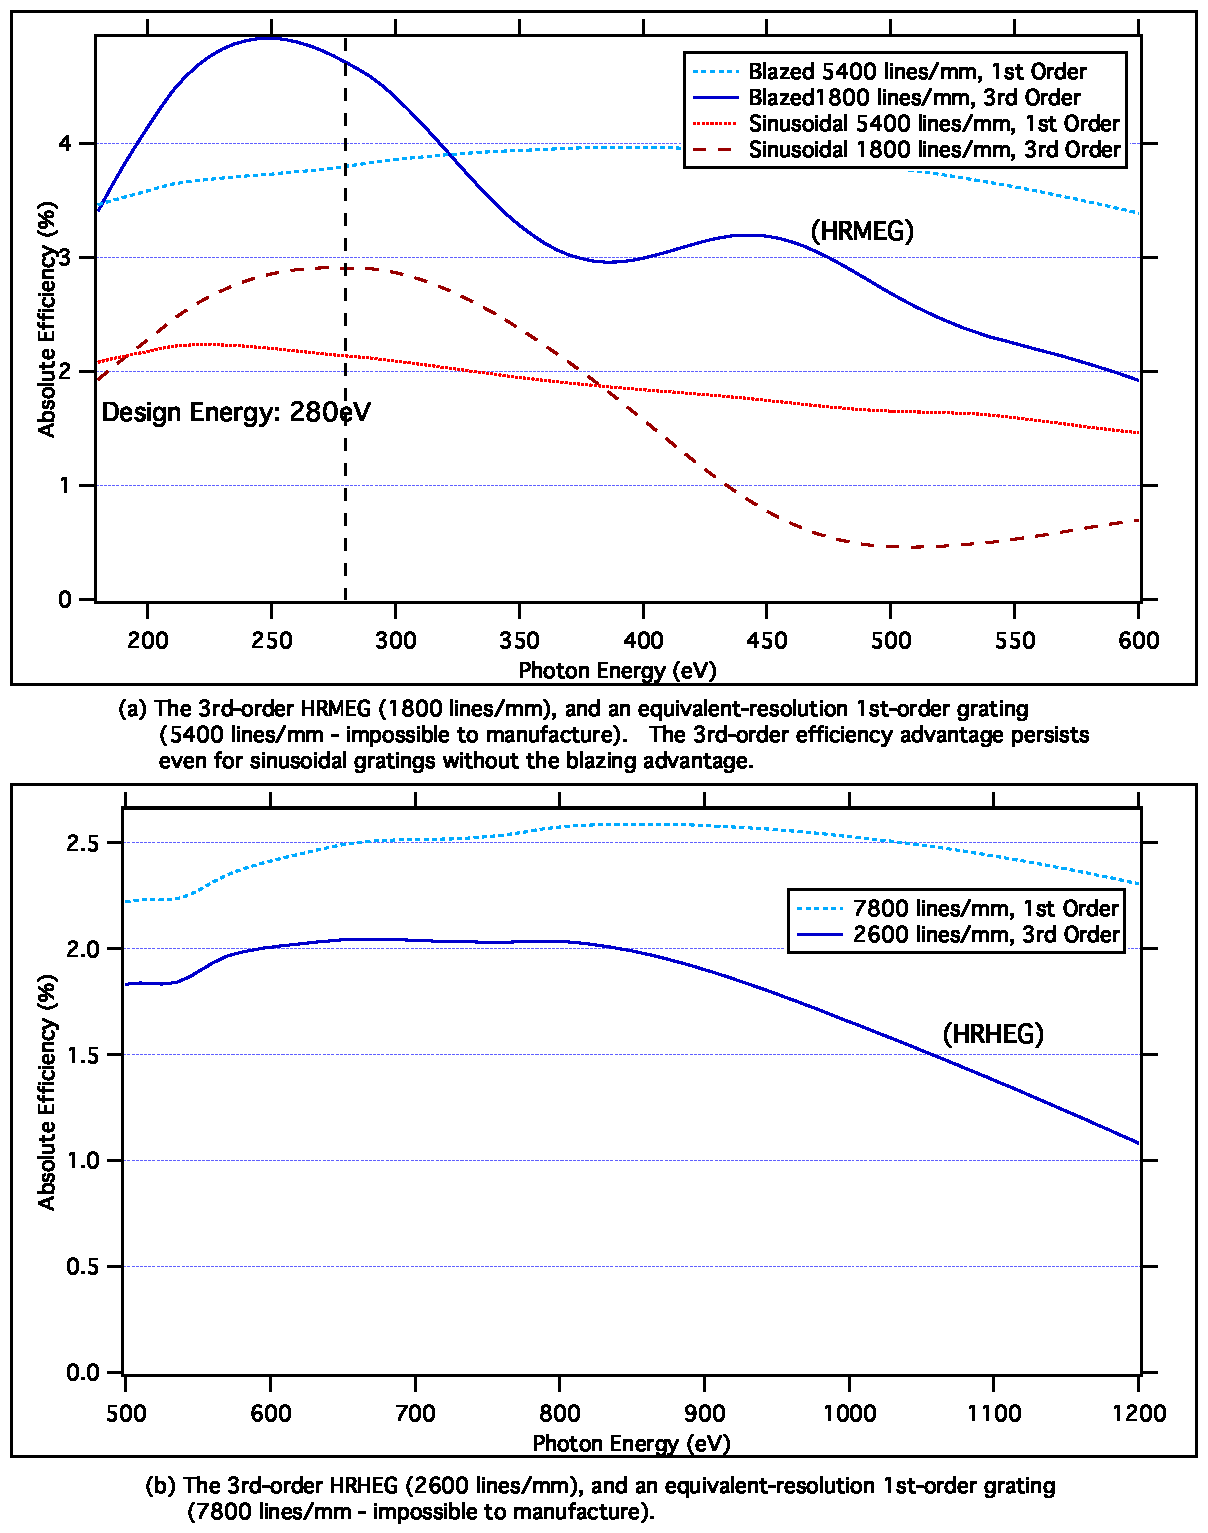
\includegraphics[scale=0.8]{Chapter4/4j_justificationFor3rdOrder/4j.pdf} 
   \caption[Justification for third-order design: At some points along the efficiency curve, the grating efficiency is actually higher in 3rd order than it would be in 1st order for an equivalent-resolution grating with three times the groove density.]{At some points along the efficiency curve, the grating efficiency is actually higher in 3rd order than it would be in 1st order for an equivalent-resolution grating with three times the groove density\ldots assuming you could even manufacture such a grating.  HRMEG and alternatives: nickel coating, geometry as indicated.  HRHEG and alternative: platinum coating, blaze angle of 4.05$\deg$.}
   \label{4e}
\end{figure}

\section{Coating choices}
Back in Chapter 5, we plotted the reflectivity and comparative efficiency for a range of common coating materials (Figure \ref{3g}, \ref{3g-2}).  From these plots it was simple to select the coating with the highest continuous reflectivity over each grating's usable energy range.  Since the IMP and MEG were only intended to be used below 800 eV, we chose a nickel coating for its high and near-constant reflectivity.  The LEG exploited the gold reflectivity peak at low energies, and we selected platinum for the remaining high-energy gratings.  (Iridium and rhodium would have provided nearly equivalent performance, but the grating manufacturer had previous experience in applying platinum coatings.)

Most of these choices proved to be optimal, but not all.  We discovered one serious consequence of using Nickel coatings, which we explore in Chapter 7.  It turns out that the surface roughness also has a significant on the real-world efficiency, so another factor in the coating choice should be how smoothly it can be applied before or after ruling.

Based on our calculations for the coating thickness (Figure \ref{3f}), we specified a conservative minimum thickness of 40 nm.

\section{Tolerancing}
The combination of efficiency and ray-tracing tools also provided a rigorous way to specify reasonable tolerances for the grating manufacturer.  Resolution criteria determined the tolerance for parameters like the groove density and grating figure.  To specify the blaze angle limits, we used calculations to determine the amount of error that would cause a 15\% relative drop from the nominal efficiency.

\section{Summary of final design}
By combining efficiency and resolution calculations to carefully manage the trade-off between these two goals, we were able to exceed our design targets of 10\% theoretical efficiency and 2000 resolving power at all the emission lines of interest, using the LEG, MEG, and HEG gratings.  The addition of the impurity (IMP) grating added extremely high efficiency over a large portion of the soft x-ray energy range, and the two 3rd order gratings added massive resolving powers of 14~000 and 10~000 at the carbon and iron lines.  (Although their efficiency is substantially lower than the other gratings, the novel usage of the 3rd order was the only way to achieve this kind of resolution within our physical size constraints.)

Table \ref{4g} shows the predicted resolving power and grating efficiency of our design for all the edges of interest.  For those interested in resolution, Figure \ref{4y} compares the resolving power of our design to the competitors in Figure \ref{4a}.  The final optimized grating parameters are included in Table \ref{gratings-table}.  In Figures \ref{4h-1} through \ref{4h-3}, we show the theoretical predicted efficiency in 1st, 2nd, and 3rd order for all six gratings.  In Chapter 7, we compare these efficiencies with the real-world diffraction performance of the manufactured gratings.

\begin{table}[h]
   \centering
   \topcaption[Predicted resolving power (RP, $E/\Delta E$) and grating efficiency (Eff) of the REIXS spectrometer at the emission lines of interest.]{Predicted resolving power (RP, $E/\Delta E$) and grating efficiency (Eff) of the REIXS spectrometer at the emission lines of interest.  Values are listed for all gratings where the emission energy lies within the detector's motion range.  (Resolving power results are adapted from Reference \cite{Mui06}.)}
   {\footnotesize
 \begin{tabular}{@{}  c cc cc cc cc cc cc @{}} % Column formatting, @{} suppresses leading/trailing space
\toprule
 	&	\multicolumn{8}{ c }{1st Order Gratings} & \multicolumn{4}{ c }{3rd Order Gratings} \\
\cmidrule(lr){2-9} \cmidrule(l){10-13}
	&	\multicolumn{2}{ c }{IMP} &	\multicolumn{2}{ c }{LEG} &	\multicolumn{2}{ c }{MEG} &	\multicolumn{2}{ c }{HEG} &	\multicolumn{2}{ c }{HRMEG} &	\multicolumn{2}{ c }{HRHEG} 		\\
	&	RP	&	Eff	&	RP	&	Eff	&	RP	&	Eff	&	RP	&	Eff	&	RP	&	Eff	&	RP	&	Eff	\\
\cmidrule(lr){2-3}   \cmidrule(lr){4-5}  \cmidrule(lr){6-7}  \cmidrule(lr){8-9}  \cmidrule(lr){10-11} \cmidrule(lr){12-13}
Si (92 eV)	&	4693	&	7.4\%	&	2986	&	38.7\%	&	10146	&	5.3\%	&	15580	&	3.6\%	&		&		&		&		\\
C (277 eV)	&	1722	&	29.1\%	&	1032	&	3.8\%	&	3646	&	19.6\%	&	5752	&	6.7\%	&	14066	&	4.7\%	&		&		\\
N (392 eV)	&	1226	&	34.1\%	&		&		&	2528	&	22.8\%	&	4039	&	9.8\%	&	10227	&	3.4\%	&	16510	&	1.5\%	\\
Fe (725 eV)	&	731	&	23.4\%	&		&		&	1588	&	17.7\%	&	1595	&	12.2\%	&	6238	&	0.9\%	&	9468	&	2.1\%	\\
\bottomrule
   \end{tabular}
   }
   \label{4g}
\end{table}

\begin{figure}[htbp] %  figure placement: here, top, bottom, or page
   \centering
   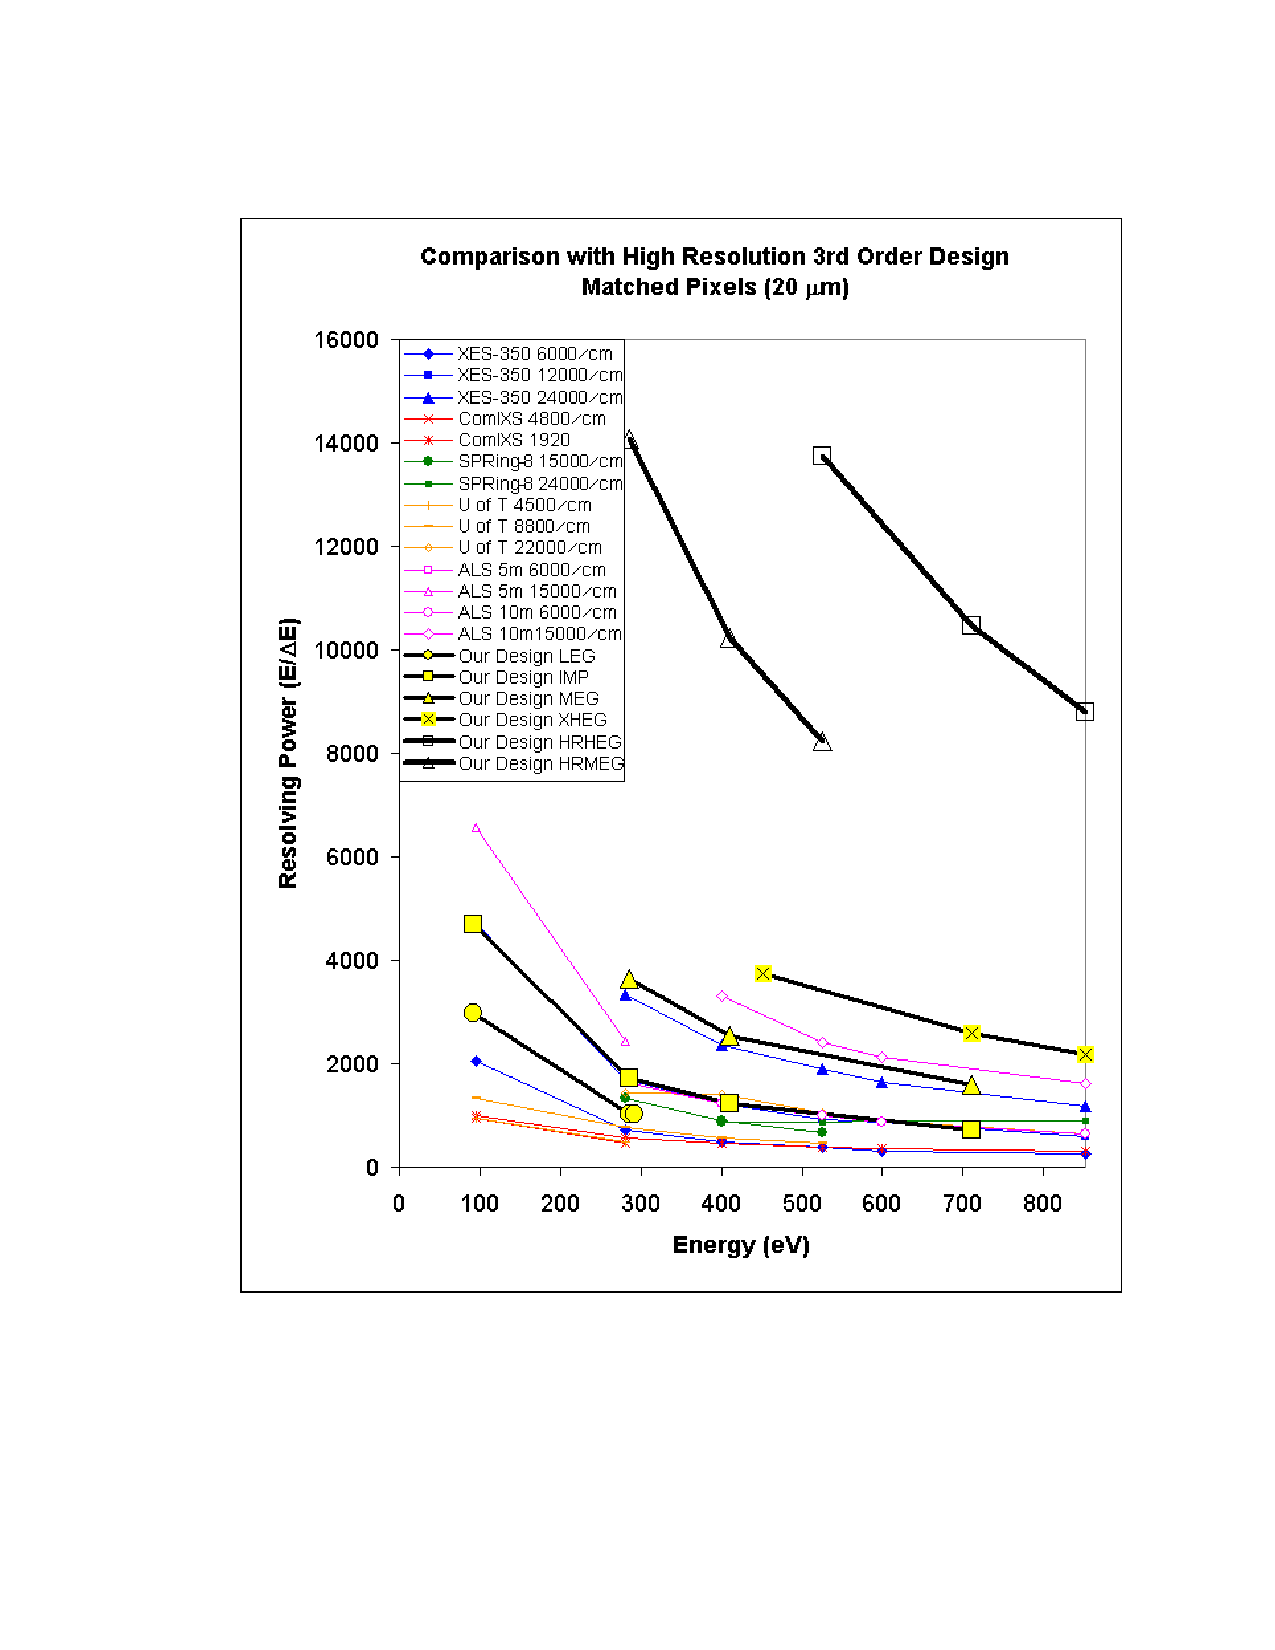
\includegraphics[scale=1]{Chapter4/4y_resolutionComparison/4y_David4_7.pdf} 
   \caption[The REIXS spectrometer design offers higher predicted resolution than the existing designs we surveyed in Figure \ref{4a}.]{The REIXS spectrometer design offers higher predicted resolution than the existing designs we surveyed in Figure \ref{4a}.  (The advantage is even more dramatic when considering the 3rd order high resolution gratings.)  However, the full strength of the design comes from a knowledgeable balance with grating efficiency, based on our combined calculations.  Reprinted from Reference \cite[Figure 4.7]{Mui06}.}
   \label{4y}
\end{figure}

\begin{figure}[htbp] %  figure placement: here, top, bottom, or page
   \centering
   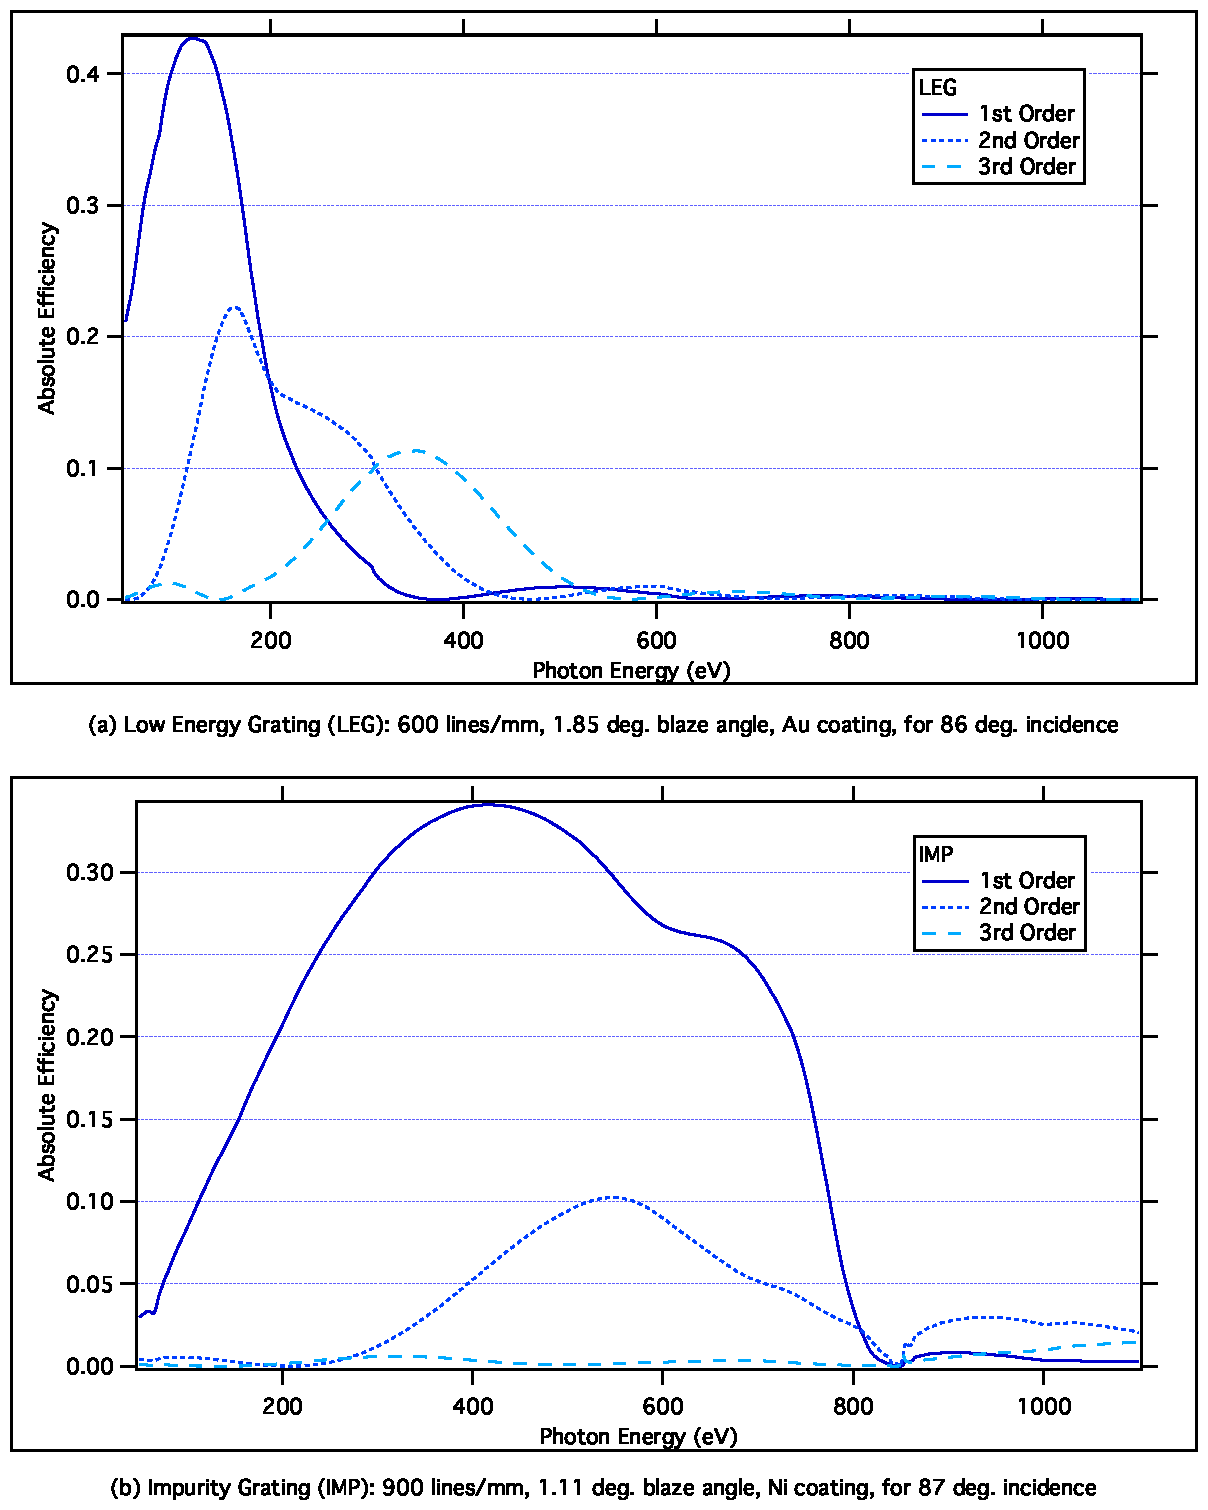
\includegraphics[scale=0.8]{Chapter4/4h_gratings/LEG_IMP.pdf} 
   \caption{Theoretical diffraction efficiency for the Low Energy Grating and Impurity Grating.}
   \label{4h-1}
\end{figure}

\begin{figure}[htbp] %  figure placement: here, top, bottom, or page
   \centering
   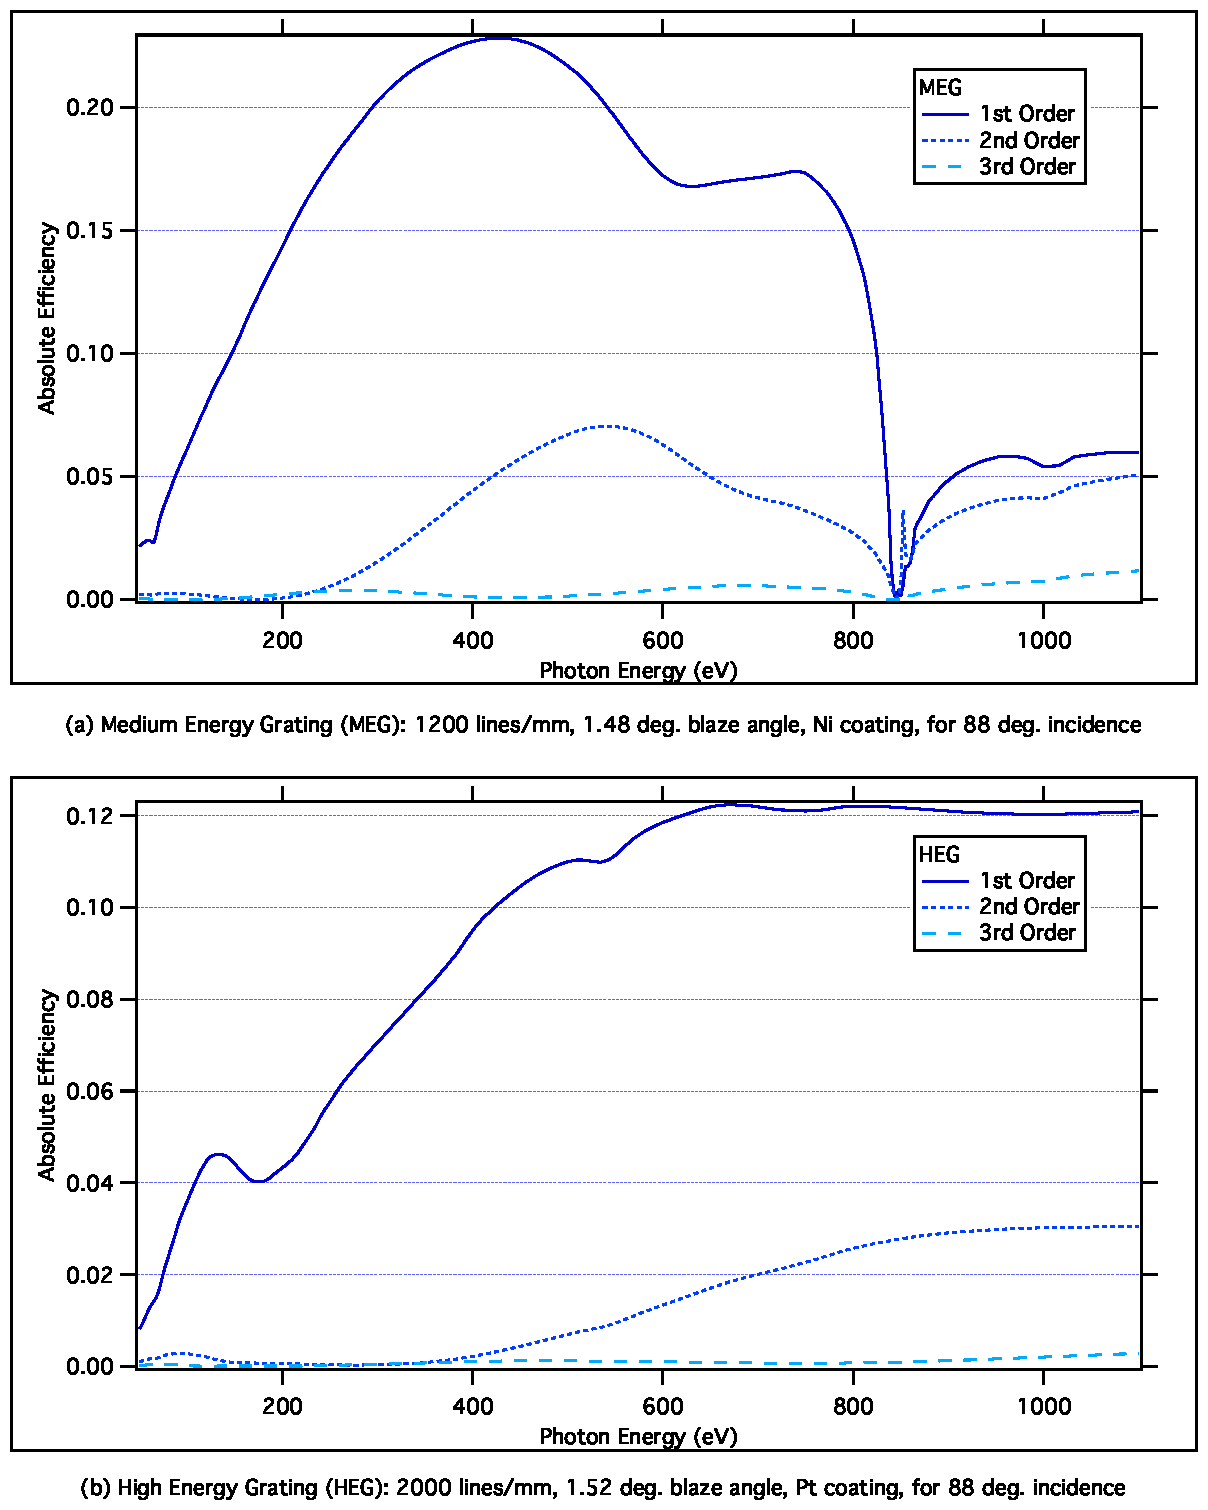
\includegraphics[scale=0.8]{Chapter4/4h_gratings/MEG_HEG.pdf} 
   \caption{Theoretical diffraction efficiency for the Medium Energy and High Energy Gratings.}
   \label{4h-2}
\end{figure}

\begin{figure}[htbp] %  figure placement: here, top, bottom, or page
   \centering
   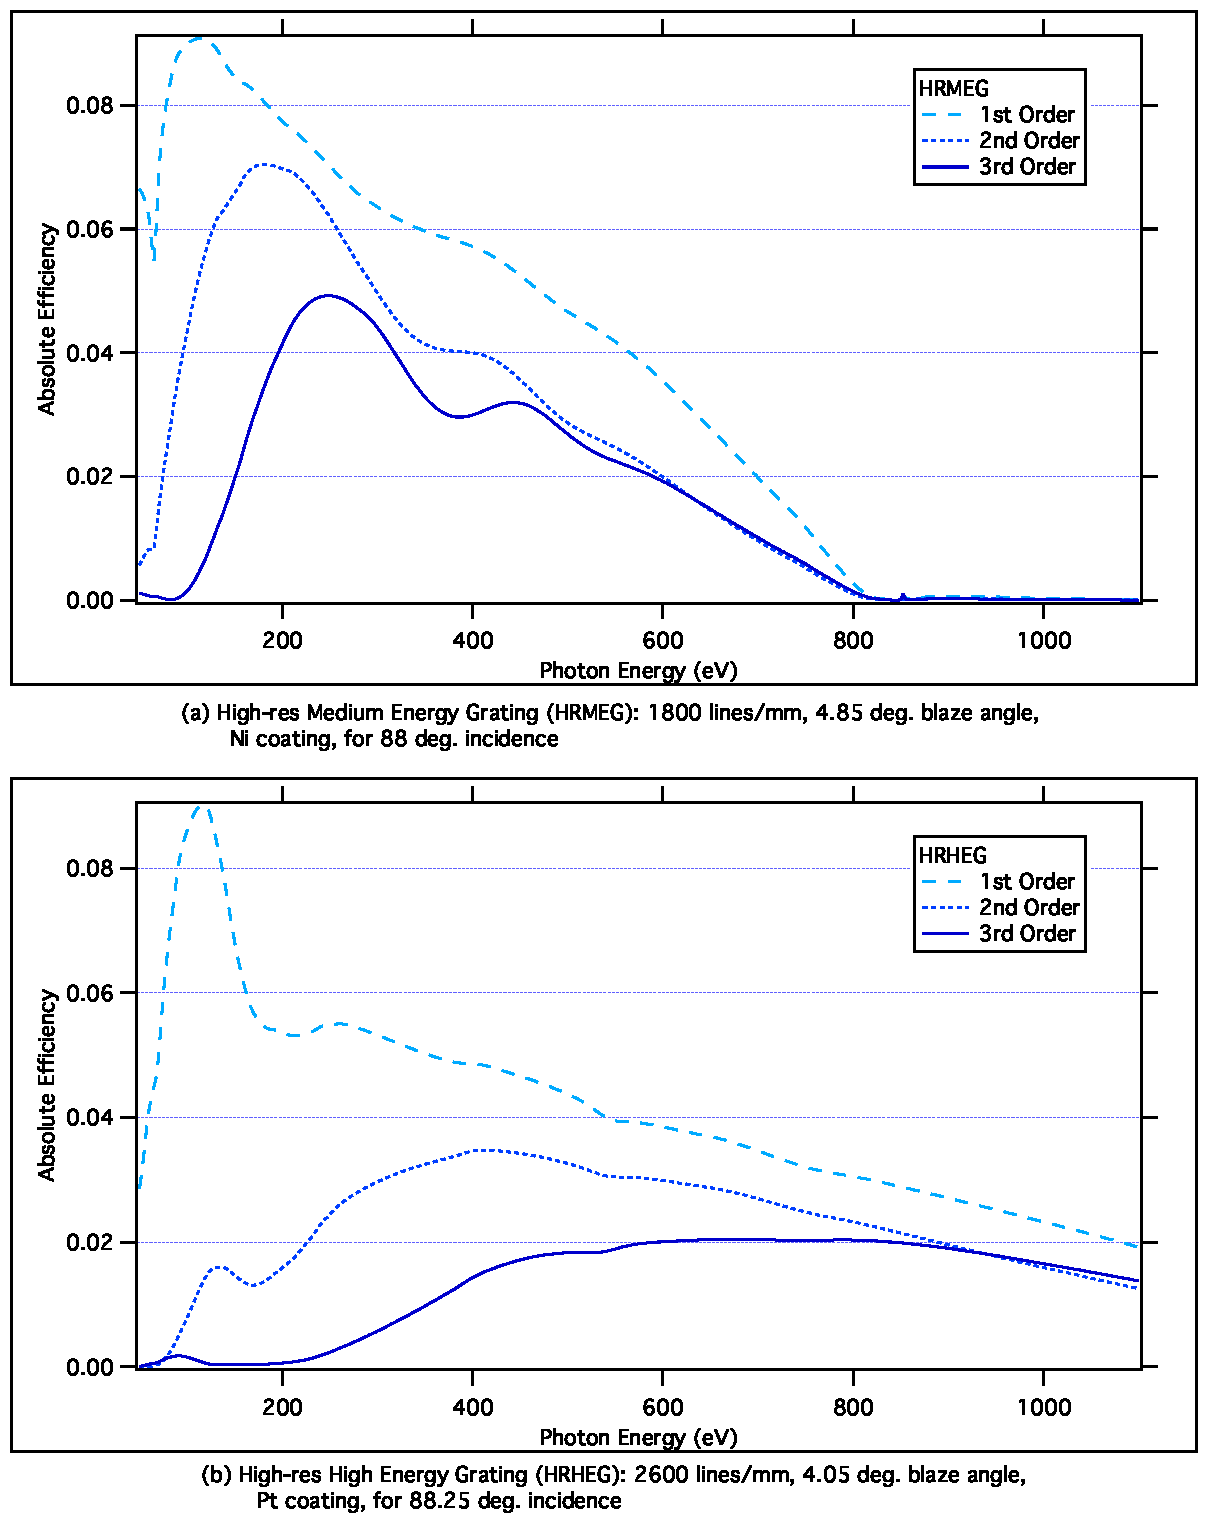
\includegraphics[scale=0.8]{Chapter4/4h_gratings/HRMEG_HRHEG.pdf} 
   \caption{Theoretical diffraction efficiency for the High Resolution Gratings, optimized to be used in 3rd order.}
   \label{4h-3}
\end{figure}